%!LW recipe=latexmk (XeLaTeX)
\documentclass[12pt,hyperref,a4paper,UTF8]{ctexart}
\usepackage{SJTUReport}
\usepackage{booktabs} % 三线表
\usepackage{amsmath}
\usepackage{amssymb} 

%%-------------------------------正文开始---------------------------%%
\begin{document}

% %-----------------------封面--------------------%%
\cover

%------------------摘要-------------%%
\newpage
\begin{abstract}

在此填写摘要内容

\end{abstract}
\newpage

\thispagestyle{empty} % 首页不显示页码

%%--------------------------目录页------------------------%%
\newpage
\tableofcontents

%%------------------------正文页从这里开始-------------------%
\newpage

%可选择这里也放一个标题
\begin{center}
   \title{ \Huge \textbf{{考虑异质用户的高速公路换电站运营MPC-RL分层协同优化}}}
\end{center}



\section{Introduction}
随着电动汽车在高速公路中长距离出行场景中的普及，沿线换电站的运营能力逐渐成为影响用户出行可靠性与系统运行效率的关键因素。相比传统充电方式，换电模式能够显著缩短车辆补能时间，但其运营过程同时受到用户到达需求、电池库存状态、充电过程和电价变化等因素影响。特别是在高速公路场景中，用户行驶路径具有明显的方向性和连续性，不同车辆到达换电站时的初始 SOC 存在差异，导致其可达站点、可行换电路径以及对站内满电电池的占用情况均不相同。因此，高速公路换电站运营本质上是一个具有时空耦合、库存动态演化和不确定需求特征的序贯决策问题。

在实际运营中，系统中存在两类异质用户，即预约用户和随机到达用户。预约用户通常提前给出出发时间、OD 路径和初始 SOC 信息，运营者需要在用户出行前对其换电站点进行合理分配，以提高服务确定性；而随机用户的到达具有更强的不确定性，运营者只能根据当前电池库存和未来需求预期决定是否服务。若仅基于当前满电电池数量进行局部决策，可能导致某些站点的满电电池被提前消耗，从而影响后续预约用户的服务可靠性；若过度保守地保留库存，则会降低随机用户服务量和系统收益。因此，如何在预约用户优先服务、随机用户灵活接纳和电池充电调度之间进行协调，是高速公路换电网络运营中的核心问题。

针对上述问题，本文构建 MPC-RL 分层协同优化框架。换电站运营中存在两类性质不同但相互耦合的决策：一类是用户服务分配决策，包括预约用户路径指派和随机用户服务量决策；另一类是充电功率决策，即不同站点、不同 SOC 电池在不同时段的充电功率安排。本文采用模型预测控制（Model Predictive Control, MPC）处理用户服务分配问题，主要原因在于该问题包含 SOC 相关可达性、网络流平衡、满电电池可用性、预约用户优先级和库存非负性等硬约束，且可行动作集合随 OD、初始 SOC 和站点库存动态变化。若直接采用 RL 进行用户指派，需要设计高维组合动作空间并处理大量动态 action masking，训练稳定性和可行性保障均较困难。相比之下，MPC 能够在滚动预测时域内显式刻画上述约束，并给出可解释、可执行的服务分配方案。

另一方面，充电功率决策虽然也可由 MPC 直接优化，但其影响具有明显的跨时段累积性：当前充电功率不仅决定当前充电成本，还会改变未来各站点不同 SOC 电池分布、满电电池供给能力和后续用户服务水平。由于充电功率动作维度相对固定，本文采用强化学习（Reinforcement Learning, RL）学习充电功率控制策略，使其能够在长期交互过程中根据需求、电价和库存状态自适应调整充电行为。如\autoref{fig:MPC-RL}所示，RL 层输出充电功率决策并影响电池状态转移，MPC 层在给定功率策略下优化预约用户和随机用户的服务分配。

进一步地，为缓解有限预测时域导致的末端效应，本文不仅使用 RL 生成充电功率动作，还利用 RL critic 提供预测时域之外的长期价值信息。传统 MPC 通常通过设置固定终端库存下界避免末端过度消耗满电电池，但该方法只能粗略限制末端满电电池数量，难以区分不同站点、不同 SOC 电池在未来需求和电价环境下的长期价值。本文在 RL 训练过程中学习状态价值函数 $V_{\theta}(s)$，并在每轮 MPC 求解前，在参考终端状态 $\bar{s}_{t+H}$ 处计算 critic 对终端库存 $w_{n,i,H}$ 的梯度，将其作为终端库存的长期边际价值系数。由此，RL 学到的长期价值被转化为 MPC 目标函数中的线性终端价值项，而无需将非线性神经网络直接嵌入优化模型。

因此，本文提出的 MPC-RL 框架并非将两个方法简单拼接，而是基于决策属性进行分层：MPC 负责处理强约束、组合结构明显且需要可解释性的用户服务分配问题；RL 负责学习具有长期影响的充电功率策略，并通过 critic 向 MPC 提供终端库存价值信息。二者通过电池库存状态、充电功率决策和终端价值项相互连接，从而在保证预约用户服务优先级和运营约束可行性的同时，使有限时域 MPC 能够近似感知预测时域之外的长期影响。

本文的主要贡献如下。xxxx【暂时不用写】

本文其余部分安排如下：第 2 节介绍 MPC 优化模型，包括时域设置、变量定义、SOC-wise expanded network 建模方法以及数学规划模型；第 3 节总结本文模型特点并讨论后续研究方向。


\begin{figure}[!htbp]
    \centering
    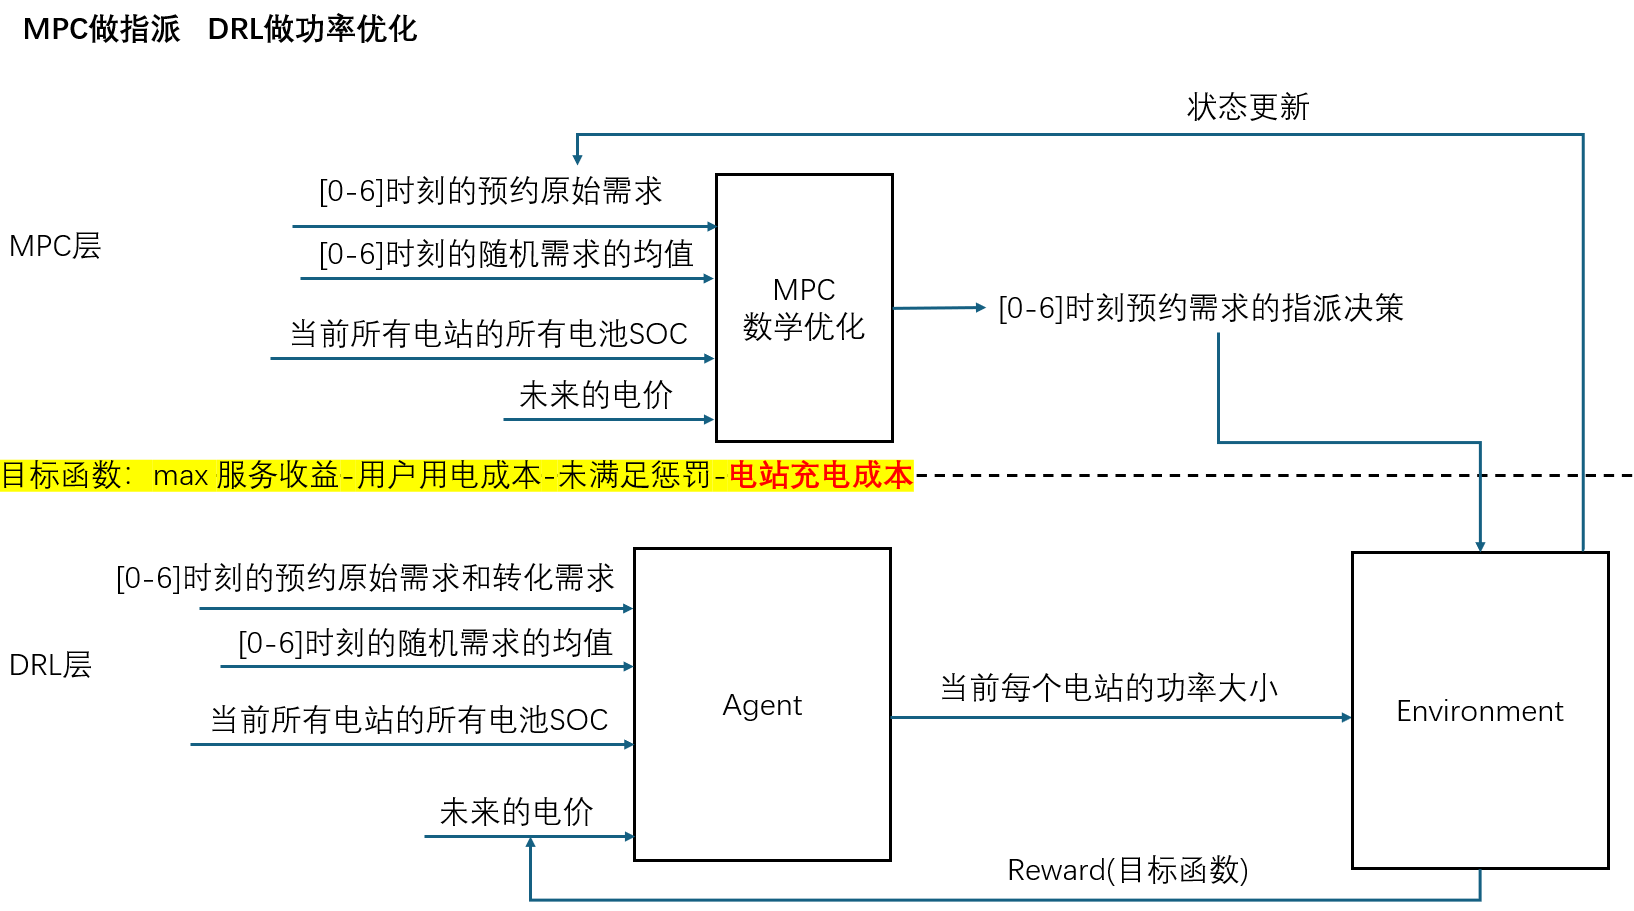
\includegraphics[width =1.0
    \textwidth]{figures/MPC-RL.png}
    \caption{MPC-RL协同优化框架}
    \label{fig:MPC-RL}
\end{figure}




\section{MPC Formulation}
\subsection{时域设置}

\begin{figure}[!htbp]
    \centering
    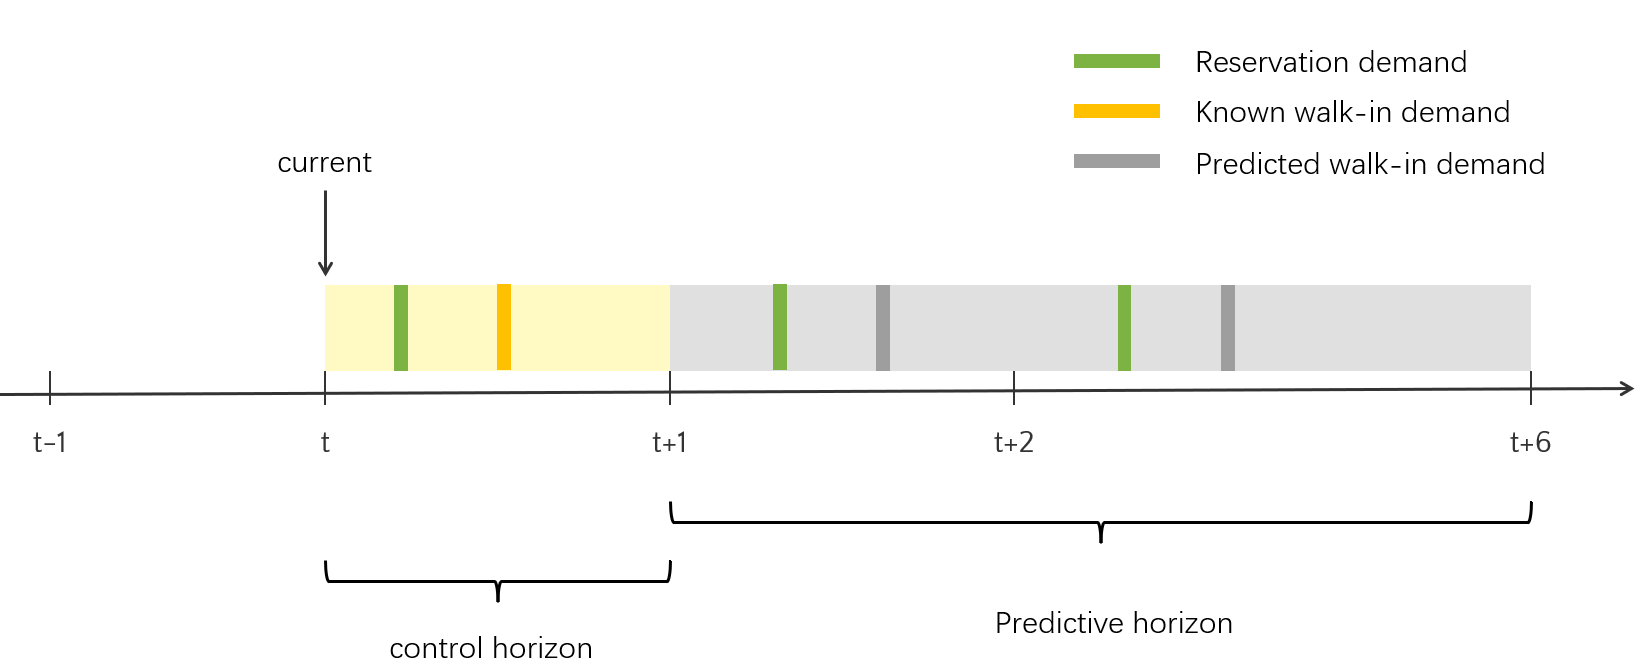
\includegraphics[width =1.0
    \textwidth]{figures/time_line.png}
    \caption{Rolling Horizon}
    \label{fig:Rolling Horizon}
\end{figure}

在t时刻，做出决策t+1时段的预约用户分配决策。

是否应该硬性保证每个预约用户都能得到服务？

\begin{itemize}
    \item 如果不硬性保证每个预约用户都能得到服务，那么存在一个风险，就是用户凭什么要预约，以及按照指派？ 在建模中使得预约用户优先级高于walk-in用户。更容易保证得到服务。或者调高惩罚参数，使得保证99\%的服务率。
    \item 如果硬性保证每个成功预约的用户都能得到服务，必须提前设置预约限制。预约限制如何设置也是一个问题。
\end{itemize}

\subsection{变量列表}

本文使用的变量如\autoref{tab:notation}所示。

% 导言区需确保已加载：
% \usepackage{booktabs}
% \usepackage{array}  % 推荐加载，增强表格功能

\begin{table}[!htbp]
  \centering
  \caption{Notation table}
  \label{tab:notation}
  \footnotesize
  \setlength{\tabcolsep}{1pt}
  \renewcommand{\arraystretch}{0.85}
  \begin{tabular}{@{}lp{13cm}@{}}
    \toprule
    \textbf{Notation} & \textbf{Description} \\
    \midrule
    \multicolumn{2}{l}{\textit{Sets and Indices}} \\
    $\mathcal{P}$ & Set of O-D pairs, indexed by $p$\\
    $\mathcal{T}$ & Set of decision time periods in predictive horizon, $\mathcal{T}:=\{1,\dots,H\}$, indexed by $t$ \\
    $\mathcal{T}^{w}$ & Set of battery inventory state time points, $\mathcal{T}^{w}:=\{0,1,\dots,H\}$, indexed by $t$ \\
    $\mathcal{N}$ & Set of charging state of batteries, $\mathcal{N}:=\{0,\dots,N\}$, indexed by $n$\\
    $\mathcal{B}$ & Set of batteries in each station, indexed by $b$ \\
    $\mathcal{S}^p$ & Set of intermediate BSSs passed through O-D pair $p$, indexed by $i, j$ \\
    $\mathcal{S}$ & Set of all BSSs in the system, $\mathcal{S}$:=$\bigcup_{p \in \mathcal{P}}\mathcal{S}^p$\\
    $\mathcal{V}^p$ & Set of nodes consisting of origin $o^p$, destination $d^p$, and all BSS $\mathcal{S}^p$ on the path of O-D pair $p$ \\  
    $\mathcal{A}^{n,p}$ & Set of arcs in battery swapping network for original state $n$, O-D pair $p$ \\
    $\mathcal{G}^{n,p}$ & Directed graph for original state $n$, O-D pair $p$, $\mathcal{G}^{n,p}:=(\mathcal{V}^p,\mathcal{A}^{n,p})$ \\
    $Path^p$ & Set of all possible paths from origin to destination for O-D pair $p$ \\
    \midrule
    \multicolumn{2}{l}{\textit{Parameters}} \\
    % $s^q$ & Origin node of demand flow $q$ \\
    % $r^q$ & Destination node of demand flow $q$ \\
    $H$ & Number of decision periods in the predictive horizon \\
    $R$ & Driving range \\
    % R^L$ & Driving range of long-range battery (km) \\
    % $N^b$ & Number of time periods required to fully charge a battery of type $b$\\
    % $N^l$ & Number of time periods required to fully charge a long-range battery \\
    $M_i$ & Number of available charging slots at station $i$ \\
    $\tau_{p,i,t}$ & The travel time of the EV departing at time $t$ arriving to station $i$ for O-D pair $p$\\
    $\tau_{p,max}$ & The maximum travel time of the EV for O-D pair $p$\\
    $P_{b,i,t}$ & Charging power of each battery $b$ in station $i$ in time period $t$\\
    $e_{i,t}$ & Electricity price at station $i$ in time period $t$\\
    $s_{i,t}$ & Service fee for battery swap of type $b$ at station $i$ in time period $t$\\
    $v^{n,p}_{i,j}$ & The amount of electricity consumed by an appointed EV with an initial charging state $n$ from station $i$ to $j$ for O-D pair $p$\\
    $v^{n}_{i}$ & The amount of electricity consumed by a walk-in EV with an initial charging state $n$ arriving at station $i$\\
    % $SOC_{b,i,t}$ & soc of battery $b$ at station $i$ in time period $t$ \\ 
    % $P_t^L$ & Service fee for long-range battery swap at time $t\in\mathcal{T}$\\
    % $P^C$ & Compensation for long-range customers swapping to standard-range battery\\
    % $c^b$ & Unit temporary configuration cost of batteries of type $b$ \\
    % $c^L$ & Unit cost of long-range battery (currency) \\
    $x_i^b$ & Initial number of batteries at station $i$ \\
    % $\hat{x}_i^L$ & Initial number of long-range batteries at station $i$ \\
    % $\bar{I}$ & Maximum battery inventory limit at each station \\
    $\alpha$ & Penalty cost per unit of unsatisfied reservation demand\\
    $\beta$ & Weight coefficient of the RL-enhanced terminal value in the MPC objective \\
    $\gamma$ & Discount factor used in RL critic training \\
    % $V_{\theta}(s)$ & RL critic/value function parameterized by $\theta$, which approximates the long-term return from system state $s$ \\
    $\bar{s}_{t+H}$ & Reference terminal state used to linearize the RL critic before solving the MPC problem \\
    $\lambda_{i,n,t}$ & Marginal terminal value of one additional battery with SOC state $n$ at station $i$, computed from the gradient of $V_{\theta}(s)$ at $\bar{s}_{t+H}$ \\
    $f_A^{n,p,t}$ & Reservation demand volume of EVs in original state $n$ for O-D pair $p$ at time $t$ \\
    $f_{R}^{n,i,t}$ & Random demand volume of EVs in original state $n$ at station $i$ in time period $t$ \\
    $\bar{y}_{A,i,j}^{n,p,k}$ & Historical service volume of reservation flows on arc $(i,j)$ that departed before the current predictive horizon, indexed by $k\in\{-\tau_{p,max},\dots,0\}$ \\
    $\bar{w}_{n,i,0}$ & Initial number of batteries in charging state $n$ at station $i$ \\
    $\underline{w}_{N,i}$ & Minimum number of fully charged batteries retained at station $i$ at the end of the predictive horizon \\
    % $\Phi^{\mathrm{RL}}_t$ & Linear terminal value term provided by the RL critic at decision time $t$ \\
    % $f_{\xi}^{L,q,t}$ & Demand volume of long-range EVs for flow $q$ at time $t$ under scenario $\xi$ \\
    \midrule
    \multicolumn{2}{l}{\textit{Variables}} \\
    % $x_i^b$ & Number of batteries of type $b$ allocated at station $i$ \\
    % $x_i^L$ & Number of long-range batteries allocated at station $i$ \\
    $y_{A,i,j}^{n,p,t}$ & Service volume of demand volume $f_{A}^{n,p,t}$ on arc $(i,j) \in A^{n,p}$, $t\in\mathcal{T}$ \\
    $y_{R}^{n,i,t}$ & Service volume of random demand volume $f_{R}^{n,i,t}$, $t\in\mathcal{T}$\\
    % $y_{i,j}^{L,q,t}$ & Service flow volume of long-range demand $f^{L,q,t}$ on arc $(i,j) \in A^{L,q}$ \\
    % $\hat{y}_{i,j}^{b,q,t}$ & Service volume of demand volume $f_{\xi}^{b,q,t}$ on arc $(i,j) \in A^{\bar{b},q}$, where $\bar{b}$ represents another battery type \\
    % $\hat{y}_{i,j}^{L,q,t}$ & Service flow volume of long-range demand $f^{L,q,t}$ on arc $(i,j) \in A^{S,q}$ (flexible swap) \\
    $w_{n,i,t}$ & Number of batteries in charging state $n$ at station $i$ at inventory state time point $t\in\mathcal{T}^{w}$ \\
    % $w_{t,n}^{l,i}$ & Number of long-range batteries at station $i$ that have been charged for $n$ periods at time $t$ \\
    % $z_{t,n}^{b,i}$ & Number of stage $n$ batteries of type $b$ at station $i$ being charged at time $t$. \\
    % $z_{t,n}^{l,i}$ & Number of long-range batteries at station $i$ being charged during period $t$ that have been charged for $n$ periods \\
    \bottomrule
  \end{tabular}
\end{table}


\subsection{soc-wised expanded network}
本文在expanded network的基础上，提出了soc-wised expanded network 建模方法，来表征不同初始SOC下的换电网络

\begin{figure}[!htbp]
    \centering
    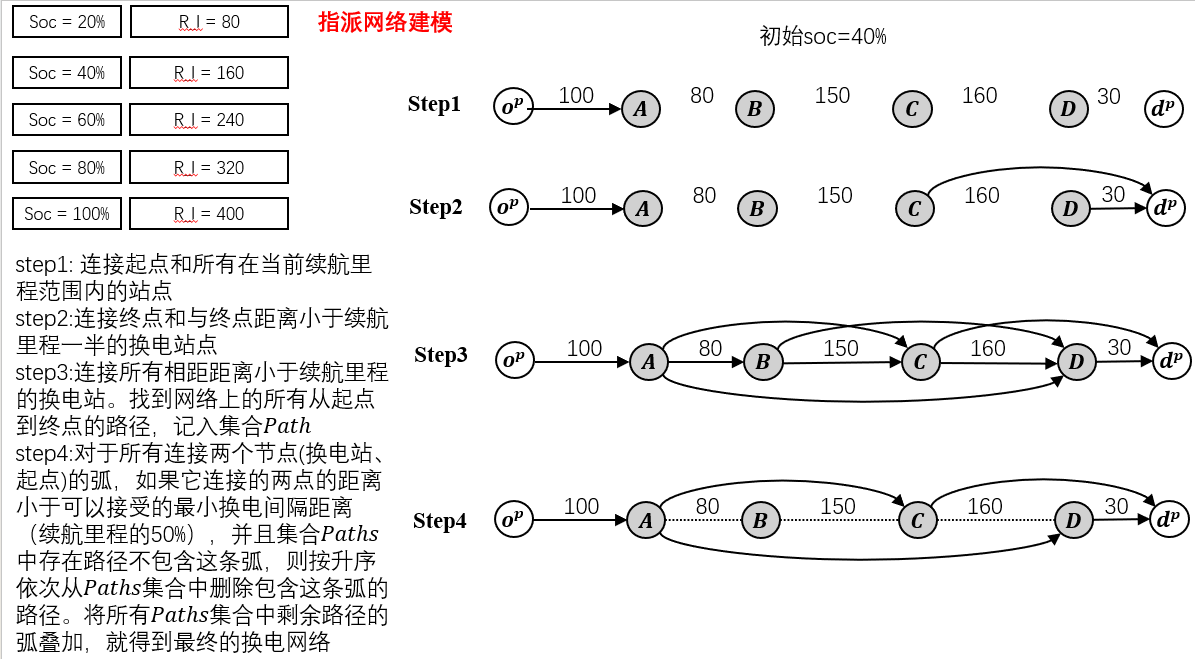
\includegraphics[width =1.0
    \textwidth]{figures/指派网络建模.png}
    \caption{指派网络建模}
    \label{fig:assignment network}
\end{figure}



\subsection{RL-enhanced terminal value approximation}

在有限预测时域 MPC 中，若目标函数仅包含预测时域内的服务收益、未满足需求惩罚和充电成本，模型可能在时域末端过度服务当前用户，从而留下对未来运营不利的电池库存状态。传统做法通常通过终端库存约束缓解该问题，但固定库存下界难以反映不同站点和不同 SOC 电池在未来需求、电价和网络位置差异下的长期价值。

为此，本文利用 RL critic 学习预测时域之外的长期价值，并将该信息以线性终端价值的形式传递给 MPC。RL 层在训练充电功率策略的同时，学习状态价值函数：
\begin{equation}
V_{\theta}(s_t)\approx
\mathbb{E}\left[\sum_{k=0}^{\infty}\gamma^k r_{t+k}\mid s_t\right],
\label{eq:critic_value}
\end{equation}
其中 $s_t$ 表示系统状态，包括各站点不同 SOC 电池库存、预约需求、随机需求预测、电价以及时间特征等；$r_t$ 与系统运营目标一致，由服务收益、未满足需求惩罚和充电成本共同决定。

由于 $V_{\theta}(s)$ 通常由深度神经网络表示，若直接将其嵌入 MPC，将导致优化模型非线性且难以由常规数学规划求解器处理。因此，本文不直接在 MPC 中使用完整的神经网络，而是在每轮 MPC 求解前，将 critic 在参考终端状态 $\bar{s}_{t+H}$ 附近进行一阶线性化。具体地，参考终端状态可由上一轮 MPC 的预测末端状态，或在给定 RL 充电功率策略下的名义滚动预测得到。在 $\bar{s}_{t+H}$ 处，有
\begin{equation}
V_{\theta}(s_{t+H})
\approx
V_{\theta}(\bar{s}_{t+H})+
\sum_{i\in\mathcal{S}}\sum_{n\in\mathcal{N}}
\lambda_{i,n,t}\left(w_{n,i,H}-\bar{w}_{n,i,H}\right),
\label{eq:value_linearization}
\end{equation}
其中长期边际价值系数定义为
\begin{equation}
\lambda_{i,n,t}
=
\left.
\frac{\partial V_{\theta}(s)}{\partial w_{n,i}}
\right|_{s=\bar{s}_{t+H}},
\quad \forall i\in\mathcal{S},\ n\in\mathcal{N}.
\label{eq:marginal_value}
\end{equation}

式\eqref{eq:marginal_value} 表示在参考终端状态附近，预测时域末端站点 $i$ 多保留一块 SOC 为 $n$ 的电池所带来的长期收益边际贡献。由于 $V_{\theta}(\bar{s}_{t+H})$ 和 $\bar{w}_{n,i,H}$ 在 MPC 求解前均为常数，不影响优化决策，因此 MPC 目标函数中仅需保留如下线性终端价值项：
\begin{equation}
\Phi^{\mathrm{RL}}_t
=
\sum_{i\in\mathcal{S}}\sum_{n\in\mathcal{N}}
\lambda_{i,n,t}w_{n,i,H}.
\label{eq:rl_terminal_value}
\end{equation}
在每次 MPC 求解时，$\lambda_{i,n,t}$ 均作为外部给定参数输入优化模型，因此终端价值项对决策变量 $w_{n,i,H}$ 保持线性，不会破坏原 MPC 模型的可求解性。若 critic 的库存输入经过归一化处理，则需将梯度按照原始库存单位进行尺度还原后再作为 $\lambda_{i,n,t}$ 使用。

\subsection{mathematical model}
目标函数为最大化预测时域内的服务收益，减去未满足预约需求惩罚和电站充电成本，并加入 RL critic 提供的线性终端价值：
\begin{equation}
\max \quad I-C_1-C_2+\beta\Phi^{\mathrm{RL}}_t
\label{eq:objective}
\end{equation}

1. 服务收益 = （预约用户+随机用户）* 服务费

\begin{equation}
I=\sum_{t \in \mathcal{T}}  \sum_{n \in \mathcal{N}} 
\left[  
% y_{A,i,j}^{n,p,t} v_{i,j}s_{i,k} + y_{R}^{n,i,t}v_is_{i,t}
% \sum_{\{k\in\mathcal{T}|k+\tau_{p,i,k}=t\}}{y^{n,p,k}_{A,i,j}}
\sum_{p \in \mathcal{P}} 
\sum_{\{(i,j) | (i,j) \in \mathcal{A}^{n,p}\}} 
\left ( y^{n,p,t+\tau_{p,i,t}}_{A,i,j}v^{n}_{i,j}s_{i,t+\tau_{p,i,t}} \right )
+\sum_{i \in \mathcal{S}} y_{R}^{n,i,t}v^n_is_{i,t}
\right]
\end{equation}

% \begin{equation}
% I=\sum_{t \in \mathcal{T}}  \sum_{n \in \mathcal{N}} 
% \left[  
% % y_{A,i,j}^{n,p,t} v_{i,j}s_{i,k} + y_{R}^{n,i,t}v_is_{i,t}
% % \sum_{\{k\in\mathcal{T}|k+\tau_{p,i,k}=t\}}{y^{n,p,k}_{A,i,j}}
% \sum_{p \in \mathcal{P}} \sum_{\{(i,j) | (i,j) \in \mathcal{A}^{n,p}\}} \sum_{\{k\in\mathcal{T}|k+\tau_{p,i,k}=t\}} \left ( y^{n,p,k}_{A,i,j}v^{n}_{i,j}s_{i,t} \right )
% +\sum_{i \in \mathcal{S}} y_{R}^{n,i,t}v^n_is_{i,t}
% \right]
% \end{equation}

% 2. 用户用电成本 = （预约用户+随机用户）* 分时用电成本
% \begin{equation}
% C_1=\sum_{t \in \mathcal{T}}  \sum_{n \in \mathcal{N}} 
% \left[  
% \sum_{p \in \mathcal{P}} \sum_{\{(i,j) | (i,j) \in \mathcal{A}^{n,p}\}} \sum_{\{k\in\mathcal{T}|k+\tau_{p,i,k}=t\}} \left ( y^{n,p,k}_{A,i,j}v^{n,p}_{i,j}e_{i,t} \right )
% +\sum_{i \in \mathcal{S}} y_{R}^{n,i,t}v^n_ie_{i,t}
% \right]
% \end{equation}

2. 未满足惩罚 = 预约用户 * 未满足惩罚
\begin{equation}
C_1 = \alpha \sum_{t\in \mathcal{T}} \sum_{p\in \mathcal{P}}  \sum_{n\in \mathcal{N}} 
\left[
f^{n,p,t}_A - \sum_{\{j | (o^p,j) \in \mathcal{A}^{n,p}\}} y^{n,p,t}_{A,o^p,j} \right]
\label{eq:penaltycost}
\end{equation}

3. 电站充电成本 = 每个站点每种规格的正在充电的电池数量*对应功率*电价
\begin{equation}
C_2 = \sum_{t \in \mathcal{T}}  \sum_{n \in \mathcal{N}} \sum_{i \in \mathcal{S}}
\left[
w_{n,i,t}P_{n,i,t}e_{i,t}
\right]
\end{equation}

4. RL 终端价值 = 预测时域末端各站点、各 SOC 电池库存 $\times$ 对应长期边际价值
\begin{equation}
\Phi^{\mathrm{RL}}_t
=
\sum_{i\in\mathcal{S}}\sum_{n\in\mathcal{N}}
\lambda_{i,n,t}w_{n,i,H}.
\label{eq:terminal_objective}
\end{equation}
其中，$\lambda_{i,n,t}$ 由式\eqref{eq:marginal_value} 在 MPC 求解前根据 RL critic 计算得到，并在本轮 MPC 优化中作为固定参数使用。

约束条件：

1. 流平衡约束
\begin{subequations}
\label{eq:flow}
\begin{gather}
\sum_{\{j| (o^p,j)\in \mathcal{A}^{n,p}\}}{y^{n,p,t}_{A,o^p,j}} \leq f^{n,p,t}_A,\quad \forall{p\in \mathcal{P},t\in \mathcal{T}},n \in \mathcal{N}\label{eq:flow1}\\
\sum_{\{j| (i,j)\in \mathcal{A}^{n,p}\}}{y^{n,p,t}_{A,i,j}} =\sum_{\{j| (j,i)\in \mathcal{A}^{n,p}\}}{y^{n,p,t}_{A,j,i}},\quad \forall{p\in \mathcal{P},t\in \mathcal{T},i\in \mathcal{S}^p}\label{eq:flow2}
\end{gather}
\end{subequations}

2. 电池状态转移约束
对soc r<N 的电池状态转移约束：

i电站t时刻soc为r的电池 = t时刻到达电站i且soc为r的预约和随机用户+t时刻充到r的电池数

t时刻充到r的电池数 = count (前面所有的电池+功率 == r )


对于预测时域开始前已经出发、但可能在当前预测时域内到达的预约车辆，其服务量在本轮 MPC 中不再作为决策变量，而是作为已知历史参数 $\bar{y}_{A,i,j}^{n,p,k}$ 进入状态转移方程，其中 $k\in\{-\tau_{p,max},\ldots,0\}$。

\begin{equation}
\begin{aligned}
w_{r,i,t}
=&
\sum_{p\in \mathcal{P}}
\sum_{n\in \mathcal{N}}
\sum_{\{j\mid (j,i)\in \mathcal{A}^{n,p}\}}
\sum_{\{k\in \mathcal{T}\mid k+\tau_{p,i,k}=t\}}
y^{n,p,k}_{A,j,i}
\mathbb{I}\!\left(N-v^{n,p}_{j,i}=r\right)
\\
&+
\sum_{p\in \mathcal{P}}
\sum_{n\in \mathcal{N}}
\sum_{\{j\mid (j,i)\in \mathcal{A}^{n,p}\}}
\sum_{\{k\in \{-\tau_{p,max},\ldots,0\}\mid k+\tau_{p,i,k}=t\}}
\bar{y}^{n,p,k}_{A,j,i}
\mathbb{I}\!\left(N-v^{n,p}_{j,i}=r\right)
\\
&+
y^{r,i,t}_{R}
+
\sum_{m\in \mathcal{N}}
w_{m,i,t-1}
\mathbb{I}\!\left(m+P_{m,i,t-1}=r\right),
\\
&\forall i\in \mathcal{S},\ r\in \mathcal{N}\setminus\{N\},\ t\in \mathcal{T}.
\end{aligned}
\tag{7a}
\end{equation}

$\mathbb{I}\!\left(N-v^{n,p}_{j,i}=r\right)$
表示预约用户在电站 i 退回的电池 SOC 为 r。

$\mathbb{I}\!\left(m+P_{m,i,t-1}=r\right)$
表示上一时刻 SOC 为 m 的站内电池，经过充电后在时刻 t 变成 SOC 为 r 的电池。

对满电电池的状态转移约束：

\begin{equation}
\begin{aligned}
w_{N,i,t}
=&
\sum_{m\in \mathcal{N}}
w_{m,i,t-1}
\mathbb{I}\!\left(m+P_{m,i,t-1}=N\right)
\\
&-
\sum_{p\in \mathcal{P}}
\sum_{n\in \mathcal{N}}
\sum_{\{j\mid (i,j)\in \mathcal{A}^{n,p}\}}
\sum_{\{k\in \mathcal{T}\mid k+\tau_{p,i,k}=t\}}
y^{n,p,k}_{A,i,j}
\\
&-
\sum_{p\in \mathcal{P}}
\sum_{n\in \mathcal{N}}
\sum_{\{j\mid (i,j)\in \mathcal{A}^{n,p}\}}
\sum_{\{k\in \{-\tau_{p,max},\ldots,0\}\mid k+\tau_{p,i,k}=t\}}
\bar{y}^{n,p,k}_{A,i,j}
\\
&-
\sum_{n\in \mathcal{N}}
y^{n,i,t}_{R},
\\
&\forall i\in \mathcal{S},\ t\in \mathcal{T}.
\end{aligned}
\tag{7b}
\end{equation}

i电站t时刻soc为N的电池 = t时刻充到N的电池数 - 换走的电池数

t时刻充到N的电池数 = count (前面所有的电池+功率 == N )

换走的电池数 = t时刻到达电站i的预约和随机用户

% \begin{subequations}
% \label{eq:transition}
% \begin{gather}
% \end{gather}
% \end{subequations}

3. 换电过程约束

由于换电站仅向用户提供满电电池，因此时刻 $t$ 电站 $i$ 可用于换电的满电电池数量为上一时刻站内电池经过充电后达到满电状态的电池数量。预约用户具有优先服务权，随机用户只能使用预约用户换电后剩余的满电电池。

\begin{equation}
\begin{aligned}
\sum_{n\in \mathcal{N}} y^{n,i,t}_{R}
&\le
\biggl[
\sum_{m\in \mathcal{N}} w_{m,i,t-1}
\mathbf{1}\!\left(m+P_{m,i,t-1}=N\right) \\
&-
\sum_{p\in \mathcal{P}}
\sum_{n\in \mathcal{N}}
\sum_{\{j\mid (j,i)\in \mathcal{A}^{n,p}\}}
\sum_{\{k\in \mathcal{T}\mid k+\tau_{p,i,k}=t\}}
y^{n,p,k}_{A,j,i} \\
&-
\sum_{p\in \mathcal{P}}
\sum_{n\in \mathcal{N}}
\sum_{\{j\mid (j,i)\in \mathcal{A}^{n,p}\}}
\sum_{\{k\in \{-\tau_{p,\mathrm{max}},\ldots,0\}\mid k+\tau_{p,i,k}=t\}}
\bar{y}^{n,p,k}_{A,j,i}\biggr]^+, \\
&\quad \forall i\in \mathcal{S},\ t\in \mathcal{T}.
\end{aligned}
\tag{8a}
\end{equation}

其中，$\sum_{m\in \mathcal{N}} w_{m,i,t-1}\mathbf{1}(m+P_{m,i,t-1}=N)$ 表示时刻 $t$ 电站 $i$ 可用于换电的满电电池数量；
第二项表示当前 MPC 决策中在时刻 $t$ 到达电站 $i$ 并需要换电的预约用户需求量；第三项表示预测时域开始前已经出发、但在时刻 $t$ 到达电站 $i$ 并需要换电的历史预约用户需求量。
该约束表示预约用户优先占用可用满电电池，随机步入用户只能使用预约用户占用后的剩余满电电池。当满电电池数量不足以满足预约用户需求时，右端为零，随机步入用户不能被服务，从而保证预约用户的优先服务权。


\begin{equation}
0\le y^{n,i,t}_{R}\le f^{n,i,t}_{R},
\qquad
\forall i\in \mathcal{S},\ n\in \mathcal{N},\ t\in \mathcal{T}.
\tag{8b}
\end{equation}

这里 (8a) 保证预约用户优先占用满电电池，(8b) 保证随机用户服务量不超过实际随机需求量。


4. 边界条件约束


为保证电池状态转移约束在时间边界处定义良好，本文区分决策变量和状态变量的时间集合。设预测时域长度为 $H$，决策时段集合为
$\mathcal{T}=\{1,\ldots,H\}$，电池库存状态时点集合为 $\mathcal{T}^{w}=\{0,1,\ldots,H\}$。
其中，服务决策变量 $y_{A,i,j}^{n,p,t}$ 和 $y_R^{n,i,t}$ 定义在 $t\in\mathcal{T}$ 上，库存状态变量 $w_{n,i,t}$ 定义在 $t\in\mathcal{T}^{w}$ 上。

首先，给定各电站在预测时域起点的电池 SOC 分布：
\begin{equation}
w_{n,i,0}=\bar{w}_{n,i,0},
\quad \forall n\in \mathcal{N},\ i\in \mathcal{S}.
\tag{9a}
\end{equation}

其中，$\bar{w}_{n,i,0}$ 表示预测时域开始时电站 $i$ 中 SOC 状态为 $n$ 的电池数量。
该约束用于初始化电池库存状态，使得后续库存状态可以由 $t=1$ 至 $t=H$ 逐期递推。

% 其次，对于预测时域开始前已经出发、但将在当前预测时域内到达的预约车辆，其服务流量不再作为当前 MPC 的决策变量，而作为历史已执行决策参数 $\bar{y}_{A,i,j}^{n,p,k}$ 进入式 (7a)、式 (7b) 和式 (8a)。因此，当 $k\leq 0$ 时，$\bar{y}_{A,i,j}^{n,p,k}$ 为已知量；当 $k\in\mathcal{T}$ 时，$y_{A,i,j}^{n,p,k}$ 为当前预测时域内的决策变量。

所有服务量和电池库存变量均应满足非负性约束：
\begin{equation}
w_{n,i,t}\ge 0,
\quad \forall n\in \mathcal{N},\ i\in \mathcal{S},\ t\in \mathcal{T}^{w},
\tag{9b}
\end{equation}

\begin{equation}
y^{n,p,t}_{A,i,j}\ge 0,
\quad \forall p\in \mathcal{P},\ n\in \mathcal{N},\ t\in \mathcal{T},\ (i,j)\in \mathcal{A}^{n,p},
\tag{9c}
\end{equation}

\begin{equation}
y^{n,i,t}_{R}\ge 0,
\quad \forall n\in \mathcal{N},\ i\in \mathcal{S},\ t\in \mathcal{T}.
\tag{9d}
\end{equation}

若需求量和电池数量均以整数计，则进一步有：
\begin{equation}
w_{n,i,t}\in \mathbb{Z}_{+},\quad
 y^{n,p,t}_{A,i,j}\in \mathbb{Z}_{+},\quad
 y^{n,i,t}_{R}\in \mathbb{Z}_{+}.
\tag{9e}
\end{equation}

% 对于时间边界，仅允许在预测时域内完成的行程进入状态转移约束。若预约用户从电站 $i$ 出发的时间为 $k$，到达时间 $k+\tau_{p,i,k}$ 超出预测时域，则对应服务变量置为零：
% \begin{equation}
% y^{n,p,k}_{A,i,j}=0,
% \quad
% \forall p\in P,\ n\in N,\ (i,j)\in A^{n,p},\
% k\in T:\ k+\tau_{p,i,k}\notin T.
% \tag{9h}
% \end{equation}

% 该约束保证所有进入电池状态转移方程的到达流均发生在当前预测时域内，避免出现到达时间超出 $T$ 后无法更新电池库存的问题。

引入 RL 终端价值后，MPC 不再仅依赖固定终端库存下界来处理末端效应。式\eqref{eq:rl_terminal_value} 通过 $\lambda_{i,n,t}$ 区分不同站点、不同 SOC 电池在未来运营中的长期边际价值，从而引导 MPC 在预测时域末端保留更有价值的库存结构。与此同时，为保证运行安全，仍可保留如下终端满电电池库存下界作为可选硬约束：
\begin{equation}
w_{N,i,H}\ge \underline{w}_{N,i},
\quad \forall i\in \mathcal{S}.
\tag{9i}
\end{equation}

其中，$\underline{w}_{N,i}$ 表示预测时域末端电站 $i$ 至少需要保留的满电电池数量。由于库存状态定义在 $\mathcal{T}^{w}$ 上，预测时域末端库存对应 $w_{N,i,H}$。在本文框架中，该约束主要作为安全库存下界，而长期影响的差异化评估由 RL critic 提供的终端价值项承担。

\section{写在最后}
\subsection{发布地址}
\begin{itemize}
    \item Github: 
    % \url{https://github.com/Jiazhen-Lei/SJTU_Course_Template_Latex}
\end{itemize}

%%----------- 参考文献 -------------------%%
%在reference.bib文件中填写参考文献，此处自动生成

\reference


\end{document}